\documentclass[11pt]{article}
\usepackage[T1]{fontenc}
\usepackage{lmodern}
\usepackage[letterpaper,margin=0.78in]{geometry}
\usepackage{amsmath,amssymb}
\usepackage{booktabs}
\usepackage{enumitem}
\usepackage{graphicx}
\usepackage{hyperref}
\usepackage{microtype}
\usepackage{tabularx}
\usepackage[most]{tcolorbox}
\usepackage{xcolor}
\usepackage{fancyhdr}

\definecolor{navy}{HTML}{172033}
\definecolor{teal}{HTML}{0F766E}
\definecolor{blue}{HTML}{2563EB}
\definecolor{orange}{HTML}{D97706}
\definecolor{purple}{HTML}{7C3AED}
\definecolor{soft}{HTML}{F1F5F9}
\definecolor{muted}{HTML}{566176}
\hypersetup{colorlinks=true,linkcolor=blue,urlcolor=blue,pdftitle={PerfSeer v3 Hardware Transfer Learning}}
\setlist{nosep,leftmargin=1.4em}
\setlength{\parindent}{0pt}
\setlength{\parskip}{0.48em}
\pagestyle{fancy}
\fancyhf{}
\lhead{\small PerfSeer v3}
\rhead{\small Hardware transfer learning}
\cfoot{\thepage}
\newcommand{\code}[1]{\texttt{\detokenize{#1}}}
\newcommand{\source}[1]{%
  \par\noindent\begin{minipage}{\linewidth}%
  \footnotesize\color{muted}\raggedright\sloppy
  \textbf{Source:} \texttt{\detokenize{#1}}\par
  \end{minipage}\par}

\begin{document}
\pagenumbering{roman}

\begin{titlepage}
  \centering
  \vspace*{1.0in}
  {\sffamily\bfseries\color{navy}\Huge PerfSeer v3 Hardware\\[0.15em]Transfer Learning\par}
  \vspace{0.35in}
  {\sffamily\Large How the teacher/student pair adapts from one NVIDIA GPU to a concrete new GPU\par}
  \vspace{0.5in}
  \begin{tcolorbox}[width=0.88\textwidth,colback=soft,colframe=teal,boxrule=0.8pt,arc=2mm]
    \centering
    \textbf{Implementation summary.} PerfSeer separates a hardware-independent graph
    workload trunk from a fixed-normalized hardware signature. For a new GPU it freezes
    the base T1 teacher and S1 student trunks, trains identity-initialized FiLM plus
    low-rank adapters on a small paired subset, learns output-specific residuals relative
    to the base GPU, and distills the target-adapted teacher into the target student.
  \end{tcolorbox}
  \vfill
  {\large Repository snapshot: \code{0db0f26082c553accb17c1d8a39802dd3d7f79fd}\par}
  {\large Architecture manifests: \code{da8ba88ed5687ce809965988b385981a9651dbc8}\par}
  \vspace{0.2in}
  {\large September 1, 2026\par}
\end{titlepage}

\tableofcontents
\newpage
\pagenumbering{arabic}

\section{Scope and evidence boundary}

This document explains the newest complete PerfSeer v3 transfer design represented by
the live \code{SeerNetV3}, training, subset-selection, artifact, and runtime code. The
selected T1/S1 model manifests were removed from the working tree by the later
labeler-only cleanup commit \code{f397092f0}; their last complete versions are preserved
in its parent, \code{da8ba88ed568}. The topology and all numerical dimensions below were
rechecked against the current source and registry rather than copied blindly from the
historical reports.

\begin{tcolorbox}[colback=orange!5,colframe=orange,boxrule=0.8pt,arc=2mm]
  \textbf{Important distinction.} ``Achieved'' here means the transfer mechanism,
  contracts, freeze controls, losses, calibration, and fail-closed artifact path were
  implemented and can be structurally verified. The repository's last transfer audit
  explicitly marked production accuracy and label-budget curves as blocked by missing
  measured A10G/target-GPU corpora and trained production artifacts. This PDF therefore
  makes no empirical ``works on any NVIDIA GPU'' claim.
\end{tcolorbox}

\section{The selected teacher/student pair}

Teacher T1 and student S1 use the same typed graph, message-passing algorithm, phase
representations, multi-task heads, and six-target order. Capacity is compressed by
reducing both hidden width and message-passing depth. Counts in Table~\ref{tab:pair}
were recomputed with the current feature layout and operation registry.

\begin{table}[h]
\centering
\caption{Current code-compatible dimensions of the selected pair.}
\label{tab:pair}
\begin{tabularx}{\textwidth}{@{}lrrrrX@{}}
\toprule
Role & Hidden & Blocks & Parameters & Target adapter & Purpose \\
\midrule
T1 teacher & 1280 & 10 & 260,114,493 & rank 32; 272,167 trainable
  & High-capacity supervised model and target-GPU teacher. \\
S1 student & 224 & 2 & 2,485,993 & rank 16; 50,615 trainable
  & CPU-deployable model distilled from the teacher. \\
\bottomrule
\end{tabularx}
\end{table}

The default target policy is \code{film_low_rank}. It updates only 0.1046\% of T1 and
2.0360\% of S1. The S1 base model itself is 0.956\% of T1 by parameter count.

\begin{center}
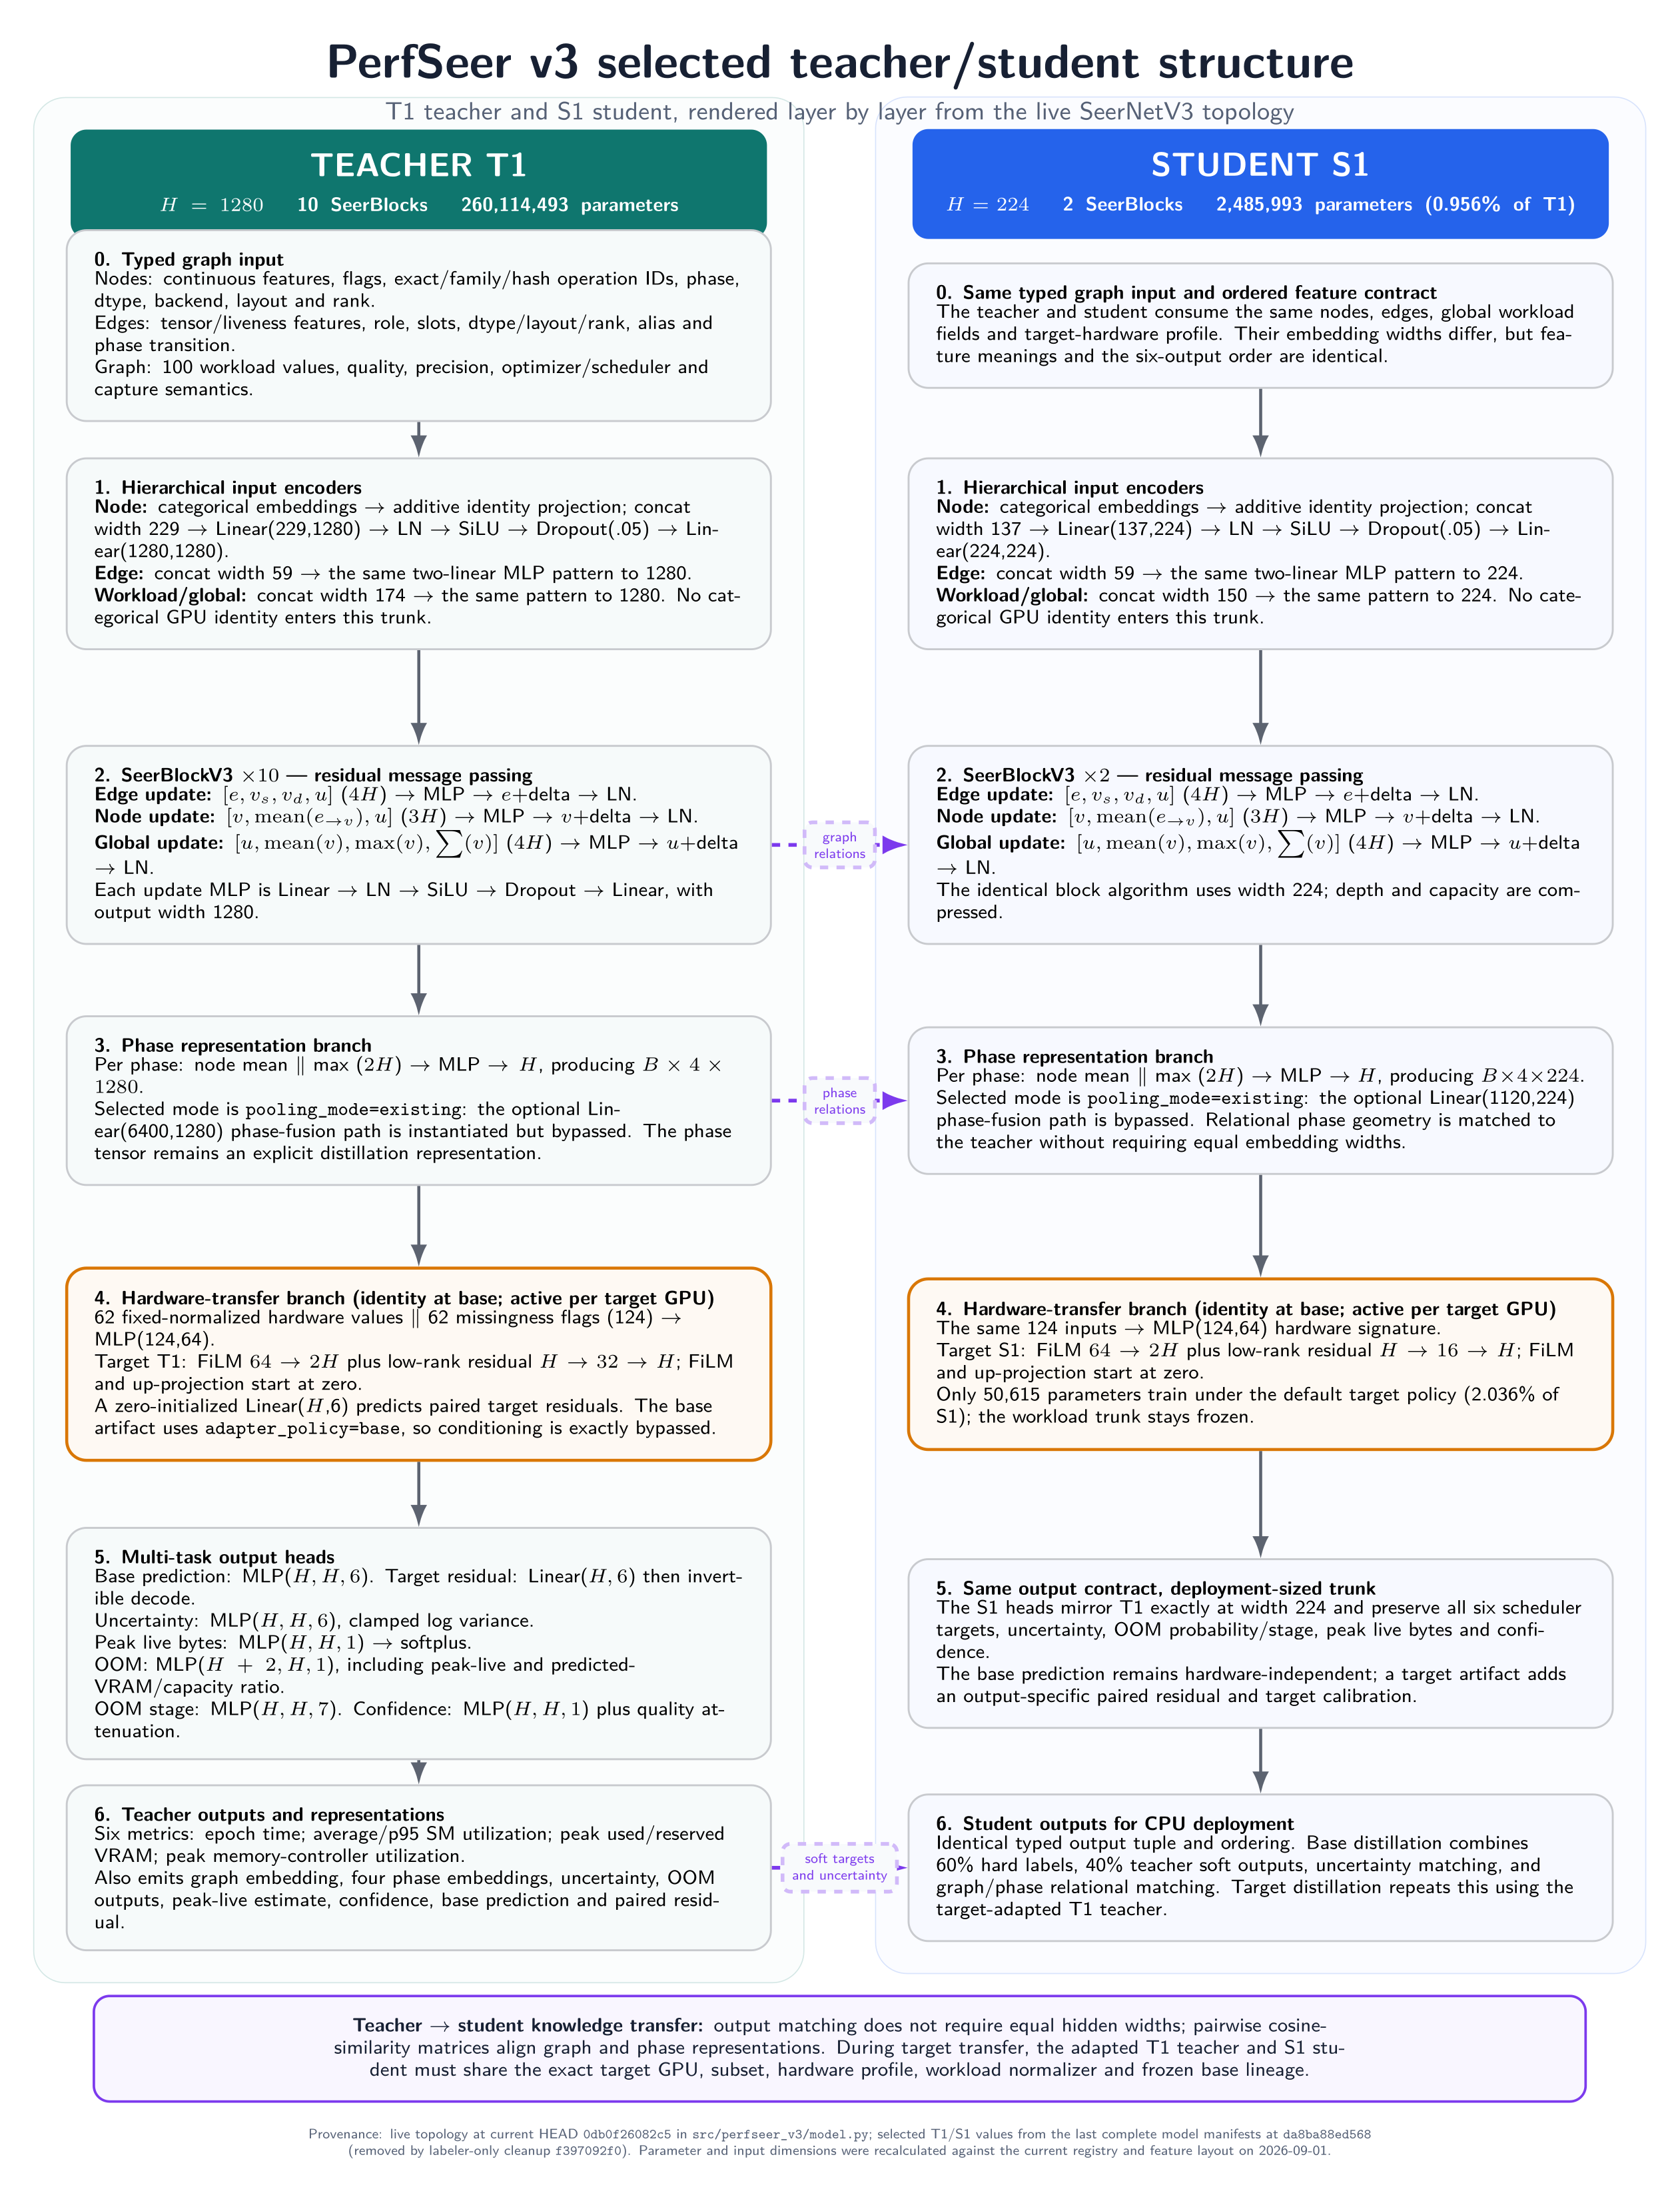
\includegraphics[width=0.98\textwidth]{teacher_student_model_structure.png}
\end{center}

\source{model.py 64--228 and 281--1048; T1/S1 manifests at Git da8ba88e}

\section{Why the architecture was split}

The design avoids learning a categorical ``GPU ID embedding'' inside the graph trunk.
Such an ID cannot describe an unseen device and encourages memorization of the base
hardware. Instead, it creates two paths:

\begin{enumerate}
  \item The \textbf{workload path} encodes operation identity, tensor/liveness edges,
  training semantics, optimizer/scheduler identity, and graph topology. Its global
  encoder is explicitly hardware-independent.
  \item The \textbf{hardware path} encodes measurable device properties. The current
  profile has 22 static and environment-compatibility fields plus 40 bounded microbenchmark
  signatures. The 62 values and 62 missingness flags form a 124-wide vector, which an
  MLP compresses to a 64-wide hardware embedding.
\end{enumerate}

Hardware values use fixed physical/reference bounds rather than statistics fitted on a
single GPU. Missing values remain visible through the mask. This makes a target profile
representable even when a particular capability or benchmark is unavailable, while
keeping workload normalization frozen from the base training split.

\source{model.py 476--629; hardware.py 17--135; features.py 241--255}

\section{End-to-end transfer procedure}

The feature is a staged pipeline, not a single fine-tuning call.

\subsection{1. Freeze a base teacher/student lineage}

The base T1 teacher is trained on hard scheduler/resource labels. S1 is then distilled
from that frozen teacher. The student combines a hard-label loss with soft teacher
outputs and relational representation matching. The selected base configuration uses
hard-label weight 0.6 and representation weight 0.05.

The base lineage binds the exact training manifest, dataset and grouped-split
fingerprints, teacher and student artifact hashes, base-teacher embedding hash, and
workload-normalization hash. A target run cannot silently substitute a different base
artifact or refit normalization.

\source{training.py 704--855; hardware_transfer.py 42--105; training_runner.py 1035--1083}

\subsection{2. Select a small, paired target subset}

The supported target budgets are 128, 256, 512, and 1,024 configurations. Their frozen
train/validation/test splits are respectively 96/16/16, 192/32/32, 384/64/64, and
768/128/128. Larger budgets must nest the immediately preceding selection.

Selection first preserves grouped split and graph-signature isolation, covers workload
strata (model family, precision, execution/resource regimes, optimizer/scheduler, and
other boundary cases), then uses farthest-point distance in \emph{base-teacher graph
embedding space}. Optional active-learning scores are allowed only after a frozen prior
subset; the test set is never chosen from model errors. A deterministic 12.5\% of the
selected set is assigned memory-boundary probing.

The same workload is measured on the base GPU and the target GPU, producing a paired
six-value label. This pairing is central: the adapter learns the hardware shift rather
than relearning the workload from scratch.

\source{hardware_transfer.py 17--39 and 115--161; transfer_subset.py 218--611}

\subsection{3. Start from an exact identity adapter}

Let $w\in\mathbb{R}^{H}$ be the workload/global embedding and
$h=\operatorname{MLP}([p,m])\in\mathbb{R}^{64}$ the target hardware embedding, where
$p$ is the normalized profile and $m$ its missingness mask. The target adapter computes

\begin{align}
  w_{\mathrm{film}} &= w + \Delta\gamma(h)\odot\operatorname{LN}(w) + \beta(h), \\
  w' &= w_{\mathrm{film}} + s\,U\,\operatorname{SiLU}(D w_{\mathrm{film}}).
\end{align}

$D$ and $U$ are the low-rank down/up projections: rank 32 for T1 and rank 16 for S1.
The FiLM weight/bias and $U$ are initialized to zero, while $s$ starts at one. The
target residual head is also zero-initialized. Consequently, before target training,
the adapted artifact is numerically the frozen base model rather than a randomly
perturbed copy.

Under \code{film_low_rank}, only the hardware-profile encoder, FiLM/low-rank adapter,
and target-residual head train. Node, edge, global, message-passing, phase, and ordinary
prediction-head parameters remain frozen. The runner hashes frozen tensors before and
after training and aborts if any byte changes.

\source{model.py 579--629 and 945--1048; hardware_transfer.py 293--359; training_runner.py 1180--1218 and 1327--1330}

\subsection{4. Learn output-specific paired residuals}

The base prediction $b$ stays hardware-independent. The adapted representation $w'$
feeds a six-value residual head $r$. Positive, scale-like outputs---epoch time, used
VRAM, and reserved VRAM (indices 0, 3, and 4)---use a log ratio:

\begin{equation}
  y_i = (b_i + \epsilon)\exp(r_i)-\epsilon.
\end{equation}

Percentage outputs---average and p95 SM utilization and peak memory-controller
utilization (indices 1, 2, and 5)---use a clipped-logit shift:

\begin{equation}
  y_i = 100\,\sigma\!\left(\operatorname{logit}
    \left(\operatorname{clip}(b_i/100,c,1-c)\right)+r_i\right),
  \qquad c=0.005.
\end{equation}

These transforms preserve positivity or percentage bounds, make zero residual exactly
recover the base prediction, and give the target adapter a relative quantity to learn.
The target teacher objective combines supervised target loss, Smooth-L1 residual loss,
identity regularization, and L2-SP regularization toward the initial adapter state.

\source{hardware_transfer.py 164--245; model.py 230--249 and 867--881; training.py 913--975}

\subsection{5. Adapt T1, then distill the target S1}

The target teacher is adapted first from the frozen base T1 artifact. The target student
then starts from the frozen base S1 artifact and learns from the already adapted T1
teacher on the same paired subset and hardware profile. Its loss combines:

\begin{itemize}
  \item hard target labels and paired residual labels (default weight 0.6);
  \item soft teacher prediction, residual, uncertainty, OOM, and OOM-stage outputs;
  \item pairwise cosine-similarity matching for graph and phase representations
  (default representation weight 0.05); and
  \item identity and L2-SP adapter regularization.
\end{itemize}

Relational matching is what permits a 224-wide student to learn representation geometry
from a 1280-wide teacher: both produce batch-by-batch similarity matrices even though
their hidden dimensions differ.

Before target-student training, the runner requires that teacher and student name the
same concrete GPU, subset hash, hardware-profile hash, workload normalizer, and frozen
base-teacher lineage. A mismatched teacher is rejected before optimization.

\source{training.py 978--1090; training_runner.py 1230--1254 and 1282--1309}

\subsection{6. Calibrate and bind a GPU-specific artifact}

After early stopping restores the best validation state, the runner fits target-specific
linear output calibration, OOM temperature calibration, and uncertainty offsets. The
artifact records the concrete target GPU allowlist plus hashes for the base artifact,
target subset, hardware profile, workload and hardware normalization policies,
calibration, paired-residual transform, adapter policy/rank, and complete transfer
lineage.

The OOM head also receives the predicted-VRAM/physical-capacity ratio explicitly, in
addition to the adapted graph embedding and predicted peak-live bytes. This makes the
capacity boundary directly visible rather than asking the model to recover it only from
an opaque embedding.

At runtime, wrong-GPU, schema, registry, capture-quality, precision, optimizer,
scheduler, training-mode, or confidence mismatches fail closed to the scheduler fallback
path.

\source{model.py 882--931; training_runner.py 1327--1428; artifact.py 137--236; runtime.py 130--285}

\section{Why this is hardware transfer learning}

The design transfers three kinds of knowledge while limiting what target labels must
teach:

\begin{itemize}
  \item \textbf{Workload knowledge is reused.} Operation semantics, graph topology, tensor
  liveness, optimizer/scheduler behavior, and phase structure remain in the frozen base
  trunk.
  \item \textbf{Hardware shift is isolated.} A measurable hardware signature conditions a small
  identity-starting adapter, and paired residuals describe how outputs move relative to
  the base GPU.
  \item \textbf{Teacher knowledge is compressed.} The target T1 teacher absorbs the new-device
  labels with more capacity; S1 learns its output behavior and relational geometry while
  retaining a small CPU-deployable architecture.
\end{itemize}

The result is a concrete-new-GPU adaptation mechanism with 128--1,024 paired labels and
a narrowly trainable parameter surface. It is deliberately not an unrestricted
full-backbone fine-tune and not a claim that one artifact generalizes to every NVIDIA
GPU.

\section{Verification performed for this rendering}

The wiki artifacts were generated only after the following checks against the current
checkout:

\begin{itemize}
  \item loaded the live operation registry and feature layout and confirmed 40 node
  continuous fields, 21 node flags, 14 edge continuous fields, 5 edge flags, 100 global
  values, 8 quality values, 62 hardware values, and 62 hardware masks;
  \item instantiated T1 and S1 on PyTorch's meta device, inspected encoder input widths,
  block counts, head dimensions, and exact parameter totals;
  \item applied the \code{film_low_rank} freeze policy and confirmed 272,167 target
  parameters for T1 and 50,615 for S1, with no workload encoder parameters trainable;
  \item checked identity initialization and paired residual encode/decode behavior;
  \item rendered the diagram at high resolution, compiled this PDF, and inspected its
  metadata, page count, embedded image, and extracted text.
\end{itemize}

\section{Source map}

\begin{tabularx}{\textwidth}{@{}lX@{}}
\toprule
Concern & Current implementation \\
\midrule
Model layers, adapters, heads, freeze groups & \path{src/perfseer_v3/model.py} \\
Hardware profile and fixed normalization & \path{src/perfseer_v3/hardware.py} \\
Transfer budgets, residuals, lineage, checksums & \path{src/perfseer_v3/hardware_transfer.py} \\
Grouped/latent subset selection & \path{src/perfseer_v3/transfer_subset.py} \\
Teacher, student, and target-adapter losses & \path{src/perfseer_v3/training.py} \\
Four-stage runner, compatibility gates, calibration & \path{src/perfseer_v3/training_runner.py} \\
Artifact integrity and runtime fallback & \path{src/perfseer_v3/artifact.py}, \path{src/perfseer_v3/runtime.py} \\
Selected T1/S1 and rank-32/rank-16 manifests & Git object \code{da8ba88ed568}: \path{src/perfseer_v3/configs/} \\
\bottomrule
\end{tabularx}

\vfill
{\footnotesize\color{muted}
Document generated from repository source. No external paper or web claim is required
for the implementation description. Historical local verification evidence is preserved
at Git object \code{da8ba88ed568}: \path{reports/perfseer_v3_transfer_completion_audit.md}.
}

\end{document}
